\documentclass[tikz,border=8pt]{standalone}
\usepackage{tikz}
\usetikzlibrary{arrows.meta,positioning,fit}
\definecolor{CourseBlue}{HTML}{315EFB}
\definecolor{CourseTeal}{HTML}{14877D}
\begin{document}
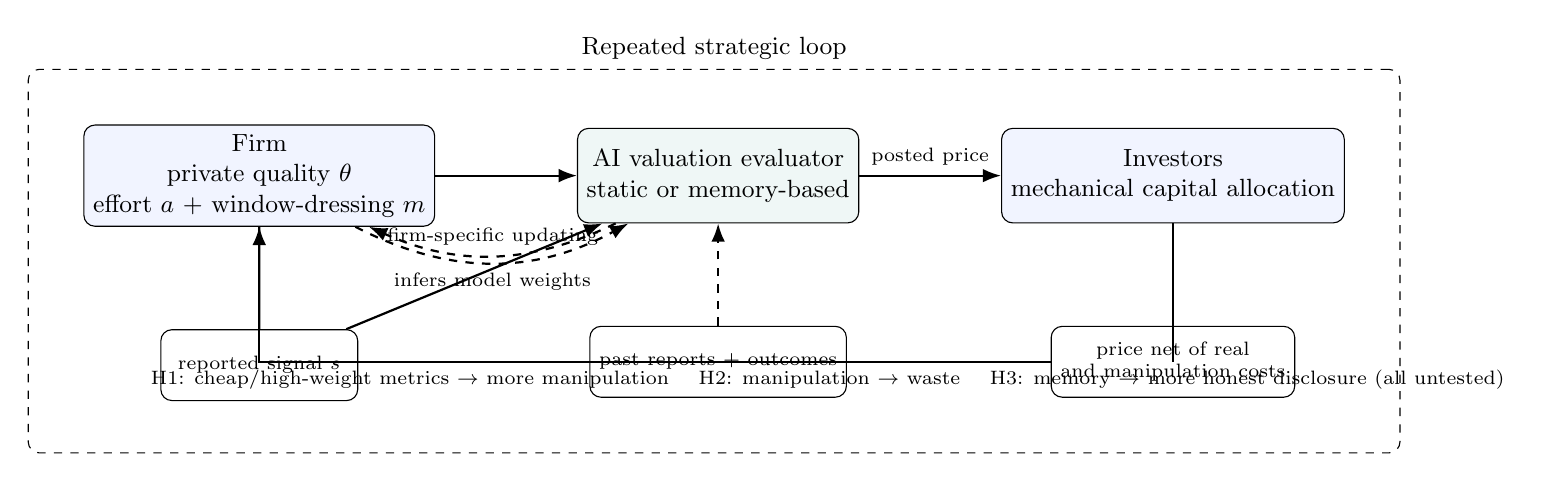
\begin{tikzpicture}[
  >=Latex,
  node distance=13mm and 18mm,
  box/.style={draw, rounded corners, align=center, minimum width=30mm, minimum height=12mm, font=\small},
  small/.style={draw, rounded corners, align=center, minimum width=25mm, minimum height=9mm, font=\scriptsize},
  arrow/.style={->, thick},
  dashedarrow/.style={->, thick, dashed}
]
\node[box,fill=CourseBlue!7] (firm) {Firm\\private quality $\theta$\\effort $a$ + window-dressing $m$};
\node[small,below=of firm] (signal) {reported signal $s$};
\node[box,fill=CourseTeal!7,right=of firm] (eval) {AI valuation evaluator\\static or memory-based};
\node[box,fill=CourseBlue!7,right=of eval] (invest) {Investors\\mechanical capital allocation};
\node[small,below=of eval] (history) {past reports + outcomes};
\node[small,below=of invest] (payoff) {price net of real\\and manipulation costs};

\draw[arrow] (firm) -- (eval);
\draw[arrow] (eval) -- node[above,font=\scriptsize]{posted price} (invest);
\draw[arrow] (invest) |- (payoff) -| (firm);
\draw[arrow] (firm) -- (signal) -- (eval);
\draw[dashedarrow] (firm) to[bend right=28] node[below,font=\scriptsize]{infers model weights} (eval);
\draw[dashedarrow] (history) -- (eval);
\draw[dashedarrow] (eval) to[bend left=25] node[above,font=\scriptsize]{firm-specific updating} (firm);

\node[draw,dashed,rounded corners,fit=(firm)(eval)(invest)(history)(payoff),
      inner sep=7mm,label={[font=\small]above:Repeated strategic loop}] {};
\node[font=\scriptsize,anchor=north west] at (-1.5,-2.35)
{H1: cheap/high-weight metrics $\rightarrow$ more manipulation \quad
 H2: manipulation $\rightarrow$ waste \quad
 H3: memory $\rightarrow$ more honest disclosure (all untested)};
\end{tikzpicture}
\end{document}